\documentclass[
11pt, % The default document font size, options: 10pt, 11pt, 12pt
%codirector, % Uncomment to add a codirector to the title page
]{charter} 




% El títulos de la memoria, se usa en la carátula y se puede usar el cualquier lugar del documento con el comando \ttitle
\titulo{Sistema de información visual para pasajeros de Trenes Argentinos} 

% Nombre del posgrado, se usa en la carátula y se puede usar el cualquier lugar del documento con el comando \degreename
\posgrado{Carrera de Especialización en Sistemas Embebidos} 
%\posgrado{Carrera de Especialización en Internet de las Cosas} 
%\posgrado{Carrera de Especialización en Intelegencia Artificial}
%\posgrado{Maestría en Sistemas Embebidos} 
%\posgrado{Maestría en Internet de las cosas}

% Tu nombre, se puede usar el cualquier lugar del documento con el comando \authorname
\autor{Ing. Carlos German Carreño Romano} 

% El nombre del director y co-director, se puede usar el cualquier lugar del documento con el comando \supname y \cosupname y \pertesupname y \pertecosupname
\director{Dr. Ing. Pablo Gomez}
\pertenenciaDirector{FIUBA} 
% FIXME:NO IMPLEMENTADO EL CODIRECTOR ni su pertenencia
%\codirector{} % para que aparezca en la portada se debe descomentar la opción codirector en el documentclass
%\pertenenciaCoDirector{}

% Nombre del cliente, quien va a aprobar los resultados del proyecto, se puede usar con el comando \clientename y \empclientename
\cliente{Trenes Argentinos Operaciones, Operadora Ferroviaria S.E.  (SOFSE)}
\empresaCliente{Empresa del cliente}

% Nombre y pertenencia de los jurados, se pueden usar el cualquier lugar del documento con el comando \jurunoname, \jurdosname y \jurtresname y \perteunoname, \pertedosname y \pertetresname.
\juradoUno{Nombre y Apellido (1)}
\pertenenciaJurUno{pertenencia (1)} 
\juradoDos{Nombre y Apellido (2)}
\pertenenciaJurDos{pertenencia (2)}
\juradoTres{Nombre y Apellido (3)}
\pertenenciaJurTres{pertenencia (3)}
 
\fechaINICIO{30 de Marzo de 2020}		%Fecha de inicio de la cursada de GdP \fechaInicioName
\fechaFINALPlan{15 de Junio de 2021} 	%Fecha de final de cursada de GdP
\fechaFINALTrabajo{12 de Diciembre de 2021}	%Fecha de defensa pública del trabajo final


\begin{document}

\maketitle
\thispagestyle{empty}
\pagebreak


\thispagestyle{empty}
{\setlength{\parskip}{0pt}
\tableofcontents{}
}
\pagebreak


\section*{Registros de cambios}
\label{sec:registro}


\begin{table}[ht]
\label{tab:registro}
\centering
\begin{tabularx}{\linewidth}{@{}|c|X|c|@{}}
\hline
\rowcolor[HTML]{C0C0C0} 
Revisión & \multicolumn{1}{c|}{\cellcolor[HTML]{C0C0C0}Detalles de los cambios realizados} & Fecha      \\ \hline
0      & Creación del documento                                 &\fechaInicioName \\ \hline
%1      & Se completa hasta el punto 4 inclusive                 & dd/mm/aaaa \\ \hline
%2      & Se completa hasta el punto 7 inclusive
%		  Se puede agregar algo más \newline
%		  En distintas líneas \newline
%		  Así                                                    & dd/mm/aaaa \\ \hline
%3      & Se completa hasta el punto 11 inclusive                & dd/mm/aaaa \\ \hline
%4      & Se completa el plan	                                 & dd/mm/aaaa \\ \hline
\end{tabularx}
\end{table}

\pagebreak



\section*{Acta de constitución del proyecto}
\label{sec:acta}

\begin{flushright}
Buenos Aires, \fechaInicioName
\end{flushright}

\vspace{2cm}

Por medio de la presente se acuerda con el Ing. \authorname\hspace{1px} que su Trabajo Final de la \degreename\hspace{1px} se titulará ``\ttitle'', consistirá esencialmente en el diseño y fabricación de un prototipo para el control de información visual para pasajeros, y tendrá un presupuesto preliminar estimado de 600 hs de trabajo y \textcolor{red}{\$XXX} de materiales, con fecha de inicio \fechaInicioName\hspace{1px} y fecha de presentación pública \fechaFinalName.

Se adjunta a esta acta la planificación inicial.

\vfill

% Esta parte se construye sola con la información que hayan cargado en el preámbulo del documento y no debe modificarla
\begin{table}[ht]
\centering
\begin{tabular}{ccc}
\begin{tabular}[c]{@{}c@{}}Ariel Lutenberg \\ Director posgrado FIUBA\end{tabular} & \hspace{2cm} & \begin{tabular}[c]{@{}c@{}}\clientename \\ \empclientename \end{tabular} \vspace{2.5cm} \\ 
\multicolumn{3}{c}{\begin{tabular}[c]{@{}c@{}} \supname \\ Director del Trabajo Final\end{tabular}} \vspace{2.5cm} \\
%\begin{tabular}[c]{@{}c@{}}\jurunoname \\ Jurado del Trabajo Final\end{tabular}     &  & \begin{tabular}[c]{@{}c@{}}\jurdosname\\ Jurado del Trabajo Final\end{tabular}  \vspace{2.5cm}  \\
%\multicolumn{3}{c}{\begin{tabular}[c]{@{}c@{}} \jurtresname\\ Jurado del Trabajo Final\end{tabular}} \vspace{.5cm}                                                                     
\end{tabular}
\end{table}


\pagebreak


\section{Introducción}
\label{sec:intro}
\subsection{Introducción específica}
El objetivo de este trabajo es desarrollar y fabricar controladores para el sistema de información visual de pasajeros (PIDS) de Trenes Argentinos (SOFSE). Este sistema se presenta al pasajero a través de carteles LED de salón que dan mensajes como la próxima estación, junto con los carteles de frente y contrafrente del tren que indican el ramal destino, como se muestra en la figura 1. 

\begin{figure}[htpb]
\centering 
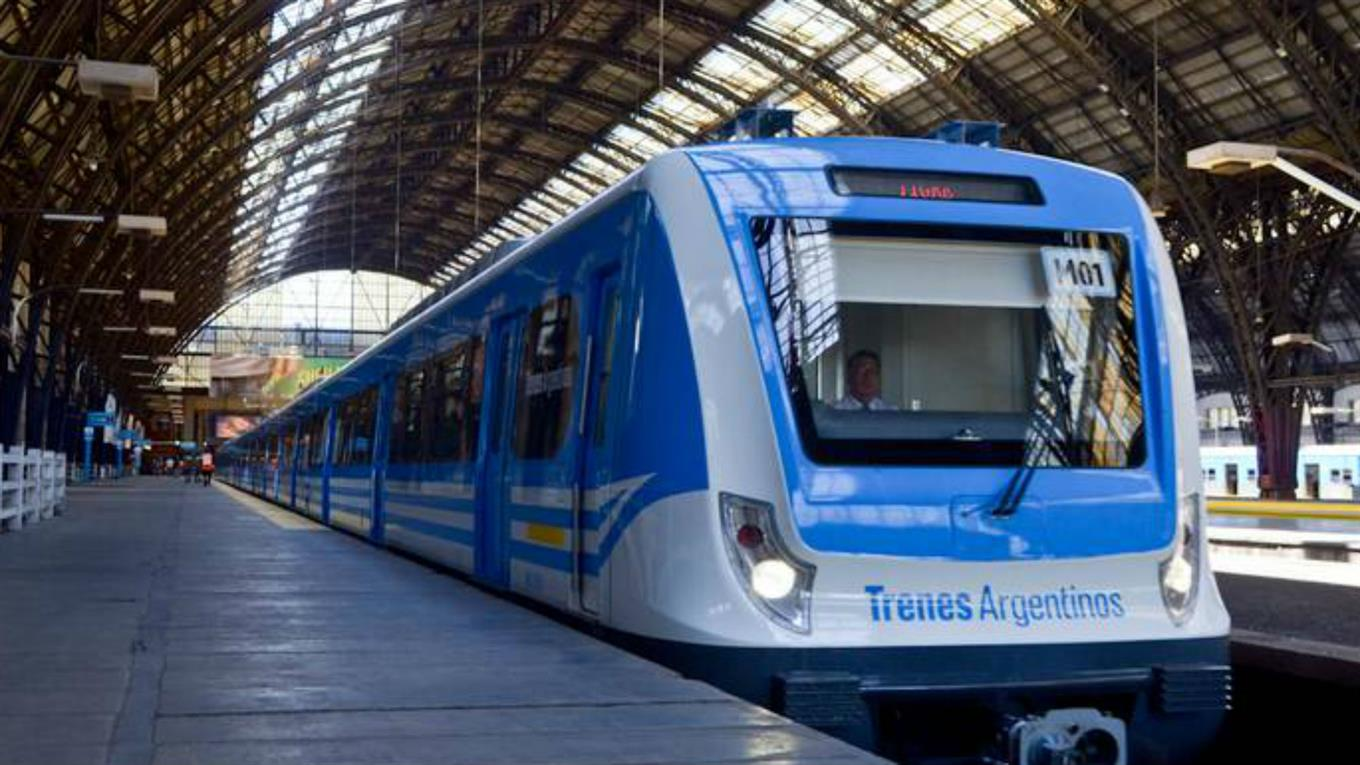
\includegraphics[width=.75\textwidth]{./Pics/tren.jpg}
\caption{Coche cabecera con la marquesina frontal que indica el destino Tigre.}
\label{fig:cartelFrente}
\end{figure}

El potencial de este trabajo es fabricar placas de control que permitan al personal de trenes realizar reparaciones y sustituir importaciones, obteniendo como resultado un mejor servicio de cara al usuario y mayor independencia tecnológica.

El desafío principal del proyecto es la compatibilidad con la red de comunicación del tren (TCN) existente. Las placas de control deben poder generar información en carteles LED y a la vez interconectarse a la red TCN. La posibilidad de fabricar el equipamiento en la industria local es también un desafío central de este proyecto.

\subsection{Antecedentes}

Survey of Development and Applicaion of Train Communication Network

El review hace un poco de historia con el origen de la red TCN.
TCN fue un tema caliente en los 90's entre Unis y empresas.
La norma de la TCN (IEC-61375) salió en el 99.
Los major players responsables de parte del estándar fueron:
* Zhuzhou Institute
* Siemens
* Bombardier
* Alstom
* Mitsubishi
En el 2008  sale la TCN basada en Real-time Ethernet


TCN define los buses jerárquicos WTB/MVB (IEC61375-2-1, IEC61375-3-1).
La especificación en capas (Física, Enlace, Red, Transmision, Aplicación) incluye:
* process data
* message data
* dynamic coupling
* addresing protocols
En los folletos de la UIC(la ITU de los trenes) aparece:
* UIC 557, UIC 647: application data y comportamiento del equipamiento onboard de:
* unidad de control de tracción
* unidad de control de puertas
* control de frenos
* UIC 556: protocolo de comunicación durante el acoplamiento de los trenes

Hay un diagrama de la TCN con 5 capas que se explica así:
-> Los operadores (conductor, staff del tren, ...) están en la capa superior. Hacen:
-> diagnóstico, tracción del tren, frenan, control de puertas, etc., (según los folletos UIC557, UIC647)
-> luego está la capa de comunicación  (folleto UIC556)
--> ésta se comunica a través de process data y message data con el WTB (IEC61375-2-1)
--> y finalmente, debajo del WTB está el MVB (IEC61375-3-1)

Bueno, hay una descripción simple en forma de tabla de WTB/MVB con los detalles de
BW, Addresing, medio físico, address space, etc.


La TCN de tiempo real basada en Ethernet sigue el esquema jerárquico y define la ETB y ECN:
ETB: Ethernet Train Backbone
ECN: Ethernet Consistent Network
La idea de esto es armar una red de  100 Mbps para:
* datos multimedia onboard
* cámaras de seguridad (2 Mbps cada una) (IEC62580-2)
* PIS (Passenger Information System) (IEC62580-4)
El perfil de comunicación (IEC61375-2-3) especifica los protocolos incluyendo
* TRDP: Train Real-time Data Protocol
Las capas física, de enlace, de red, transmisión y aplicación están en
* IEC61375-2-5 (ETB) y IEC61375-3-4 (ECN)

Igual que antes, un diagrama de capas explica el funcionamiento de la ETB/ECN:
-> Los operadores (conductor, staff del tren, ...) están en la capa superior. Hacen:
-> diagnóstico, tracción del tren, frenan, control de puertas, CCTV, PIS,
(según los perfiles de aplicación IEC61375-2-4, IEC62580-2...)
-> luego está la capa de comunicación  (IEC61375-2-3)
--> ésta se comunica a través de process data y message data con el
Train  Backbone Network Standard (IEC61375-2-5)
--> y finalmente, debajo está el Train Marshalling network Standard (IEC61375-3-4)


Les dejo las tablas:

| WTB | MVB
----------------------------------------------------------------------
Networking mode | Auto  dynamic | Determined in advance |
Physical medium | Shielded par tr.| Shielded par tr. |
Comm. Dist. | 860 m | 20 m (ESD), 200 m (EMD) , 2000m (OGF) |
Signal | Manchester codes with 16...32 | Manchester codes with |
| preamble code | delimiters |
Bandwidth | 1 Mbps | 1.5 Mbps |
Address space | 8 bit address | 12 bit addr.|
Length of frame | range:4–132 byte| 2, 4, 8, 16, 32 bytes |
Addressing mode | Dynamic | Static addressing |
Typical cycle | 25 ms | 16 ms |
Redundancy mode | A/B line | A/B line |
Media access | Master and slave| Master and slave |
Real-time prot. | TCN real-time protocol | - |
-------------------------------------------------------

| ETB | ECN |
-------------------------------------------------------
Networking mode | Auto  dynam| Determined in adv.|
Physical medium | Cat5e par   | Cat5e par  |
Commu. distance | 100 m | 100 m  |
Bandwidth | 100 Mbps | 100 Mbps  |
Packet length | 1500 Bytes | 1500 Bytes  |
Addressing mode | Dynamic | Static  |
Typical cycle | 10 ms | 10 ms |
Minimum cycle | 4 ms | 1 ms |
Redundancy mode | Link aggr.n | Ring |
Media access | CSMA/CD | CSMA/CD |
Network layer | IPV4 | IPV4 |
Transm. layer | UDP multicast/unicast, TCP | UDP multicast/unicast, TCP |
Real-time prot. | TRDP | – |
App layer serv | DHCP, DNS, SNTP, SNMP | DHCP, DNS, SNTP, SNMP |
-------------------------------------------------------------------------

\pagebreak

\section{Planificación}

\pagebreak

\section{Diseño}

\subsection{Display LED}
La placa de control del display LED matricial se representa con el diagrama de bloques de la figura \ref{fig:blockDiagram LED display}. La entrada es un conector de dieciséis pines (2x8) que entrega señal de datos a dos transceivers 74HC245D. El circuito de los transceivers s

\begin{figure}[htpb]
\centering 
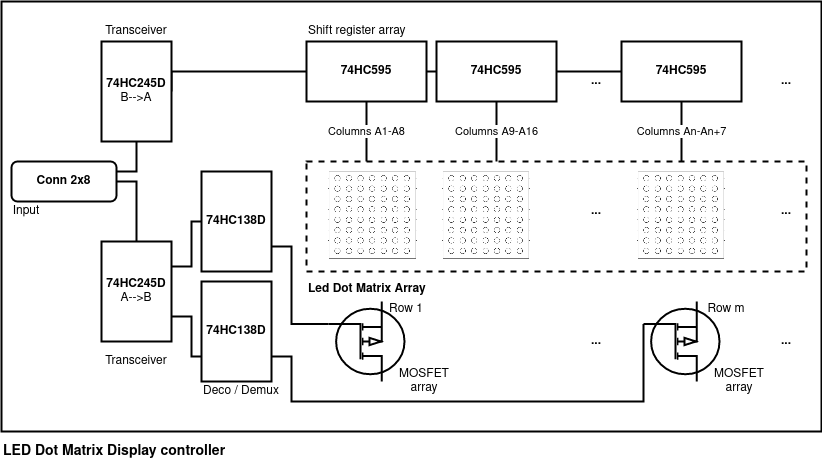
\includegraphics[width=1\textwidth]{./Pics/blockDiagram.png}
\caption{Diagrama de bloques del controlador del display LED.}
\label{fig:blockDiagram LED display}
\end{figure}

\subsection{Controlador}


\subsection{Firmware}

\subsubsection{Máquinas de estado (fsm)}
El sistema de visualización de mensajes será el encargado de recibir información por parte de un sistema mayor (red TCN) y de presentar información al pasajero a través de carteles LED. Dado que el sistema completo es un Tren y su función es transportar pasajeros a lo largo de un recorrido o ruta de
estaciones, se ha modelado la visualización de mensajes del sistema  utilizando el patrón de máquinas de estado. El diseño de pruebas entonces aprovecha este patrón con las técnicas de STT
(State Transition Testing). A continuación se detalla paso a paso el diseño de las pruebas de sistema y de aceptación. 

En la figura \ref{fig:Statechart} se describe la máquina de estados del subsistema Parte B. Los estados posibles
del sistema son:
\begin{itemize}
\item \textbf{Detenido}: el tren está detenido en las cabeceras o en algún punto de su ruta.
\item \textbf{Cabecera}: el tren se encuentra en una estación cabecera de su ruta.
\item \textbf{Circulando}: el tren está viajando a velocidad constante a lo largo de su ruta.
\item \textbf{Arribando}: el tren está viajando con velocidad decreciente (frenando) a lo largo de su
ruta.
\item \textbf{Estación}: el tren se encuentra en una de las estaciones de su ruta
\end{itemize}

\begin{figure}[htpb]
\centering 
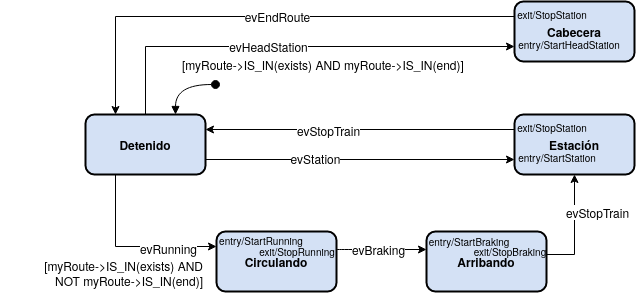
\includegraphics[width=1\textwidth]{./Pics/Statechart.png}
\caption{Máquina de Estados del sistema.}
\label{fig:Statechart}
\end{figure}

Los eventos de transición entre cada estado se presentan en la figura \ref{fig:State tree} y se detallan a continuación:

\begin{itemize}
\item \textbf{evStopTrain}: señal de tren detenido. No presenta mensajes al pasajero.
\item \textbf{evStation}: el tren se encuentra en una estación. Se presenta al pasajero el nombre de
la estación y la información relevante a la misma.
\item \textbf{evRunning}: señal de circulación, el tren comienza a acelerar hasta alcanzar una
velocidad constante. No presenta mensajes al pasajero.
\item \textbf{evBraking}: señal de frenado, el tren comienza a frenar para detenerse en una estación.
Se presenta al pasajero la información de la próxima estación.
\item \textbf{evEndRoute}: señal de final de recorrido. Se presenta el mensaje de que el tren ha
llegado a la estación cabecera.
\item \textbf{evHeadStation}: señal de cabecera. Se presenta la información relativa a la estación cabecera y a la próxima ruta.
\end{itemize}

En la tabla se detallan las transiciones entre estados posibles. Los números referencian las pruebas a realizar.

\begin{figure}[htpb]
\centering 
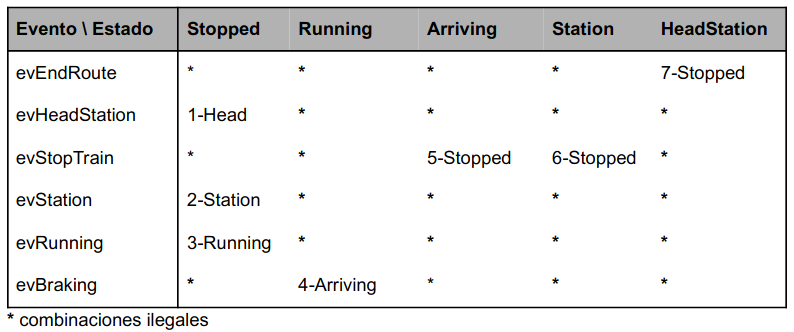
\includegraphics[width=1\textwidth]{./Pics/TablaStatechart.1.png}
\caption{Tabla de transiciones de estados.}
\label{fig:State transition table}
\end{figure}

El estado inicial del tren es Detenido, y corresponde a la raíz del árbol de la figura \ref{fig:State tree}:

\begin{figure}[htpb]
\centering 
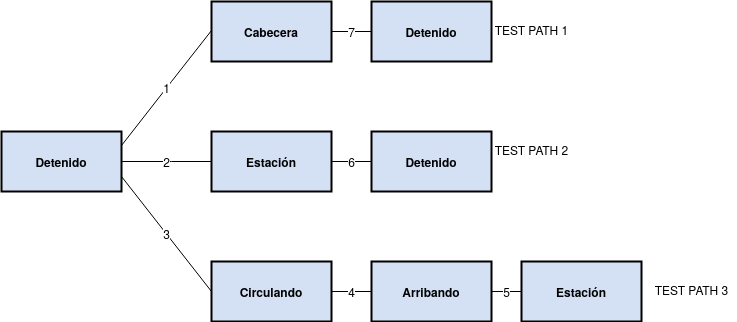
\includegraphics[width=1\textwidth]{./Pics/STT.Tree.png}
\caption{Árbol de transiciones de estados.}
\label{fig:State tree}
\end{figure}

Los casos de prueba legales, es decir aquellos que corresponden a
transiciones entre estados posibles en el sistema se detallan en la sección de Pruebas e integración.





\pagebreak
\subsubsection{Sistema operativo de tiempo real(RTOS)}

\pagebreak
\section{Fabricación}
\pagebreak
\section{Pruebas de integración}
\subsection{Análisis de los protocolos de comunicación}

\begin{figure}[htpb]
\centering 
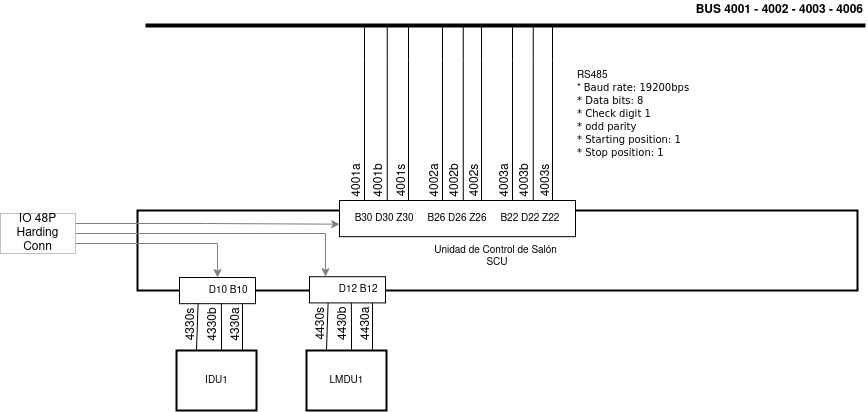
\includegraphics[width=1\textwidth]{./Pics/RedPIDS.drawio.png}
\caption{Diagrama del plano esquemático del punto de medición.}
\label{fig:test point SCU-PIDS diagram}
\end{figure}


\begin{figure}[htpb]
\centering 
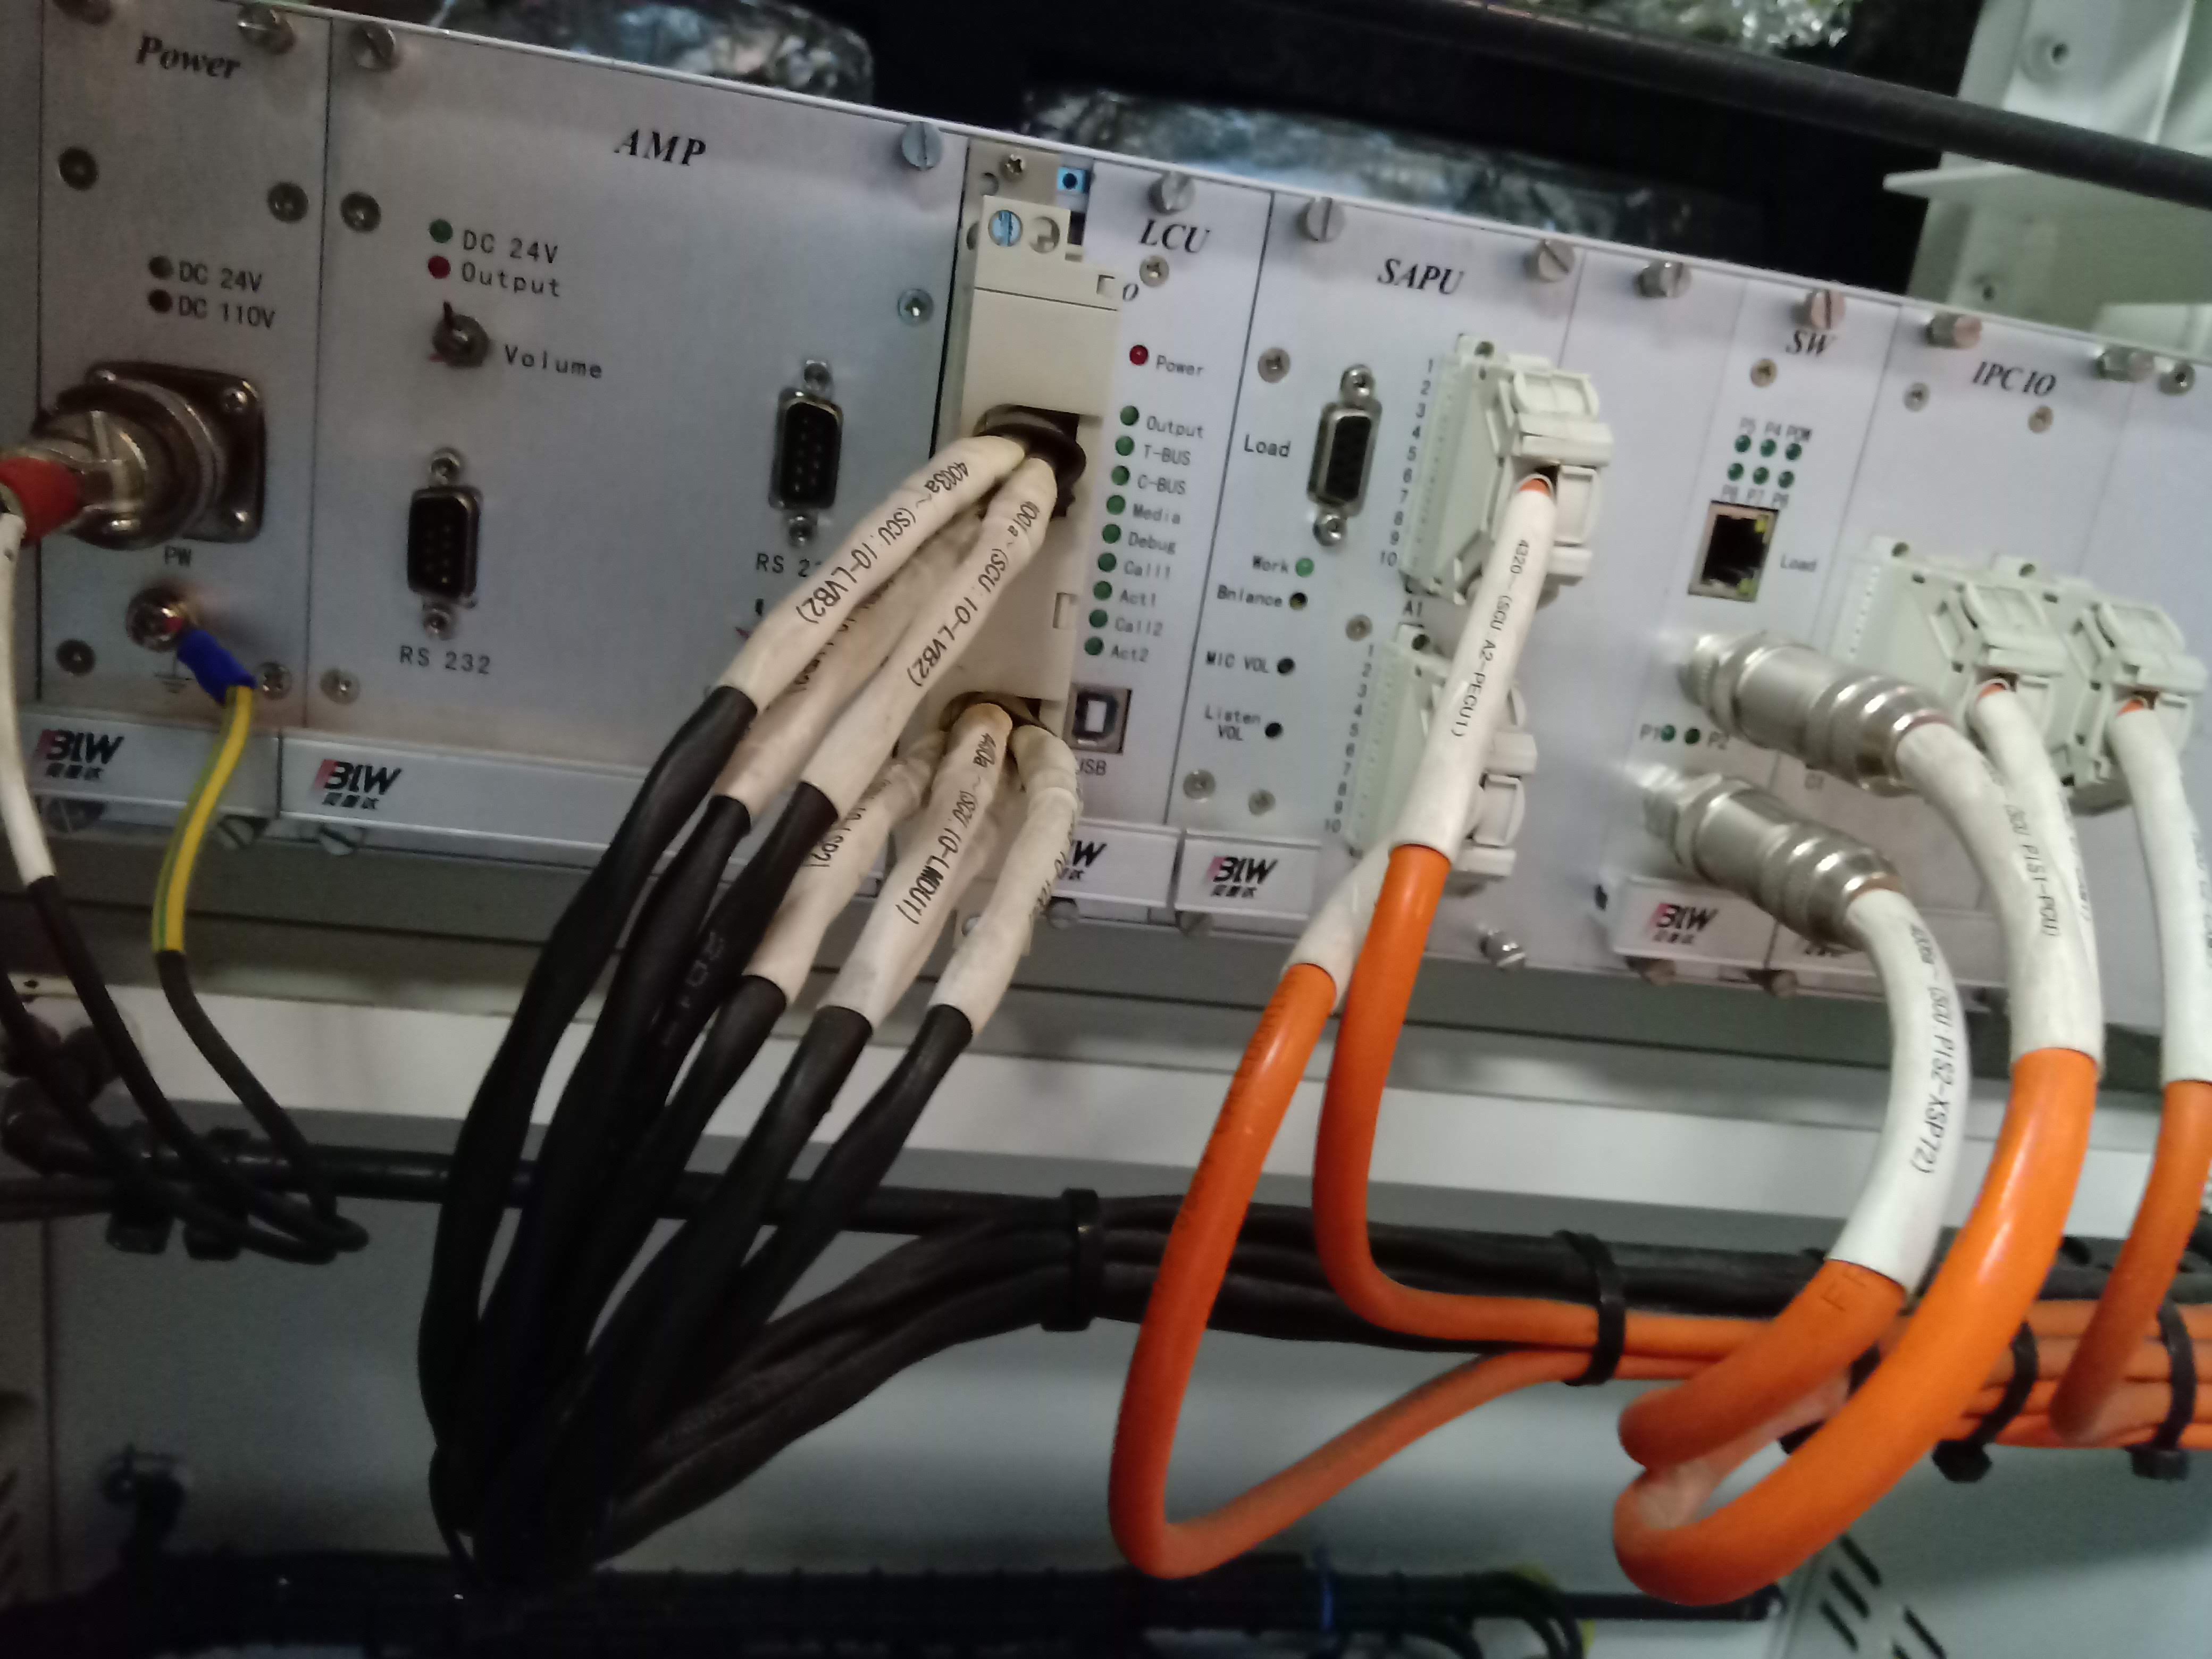
\includegraphics[width=1\textwidth]{./Pics/IMG_20210322_122403.jpg}
\caption{Fotografía del punto de medición a intervenir para realizar capturas.}
\label{fig:NOsniffingPhoto}
\end{figure}



\begin{figure}[htpb]
\centering 
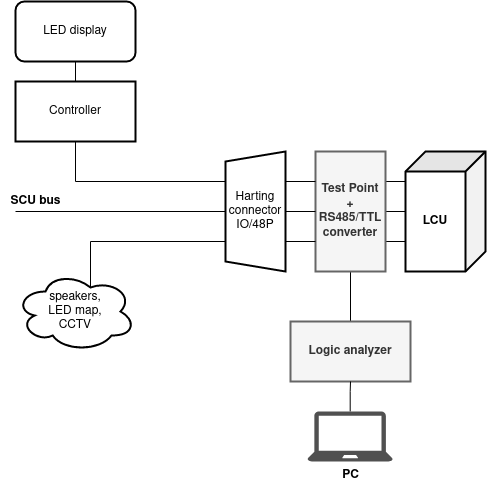
\includegraphics[width=1\textwidth]{./Pics/sniffingDiagram.drawio.png}
\caption{Diagrama de bloques del ensayo para el análisis de protocolos de comunicación.}
\label{fig:sniffingDiagram}
\end{figure}

\begin{figure}[htpb]
\centering 
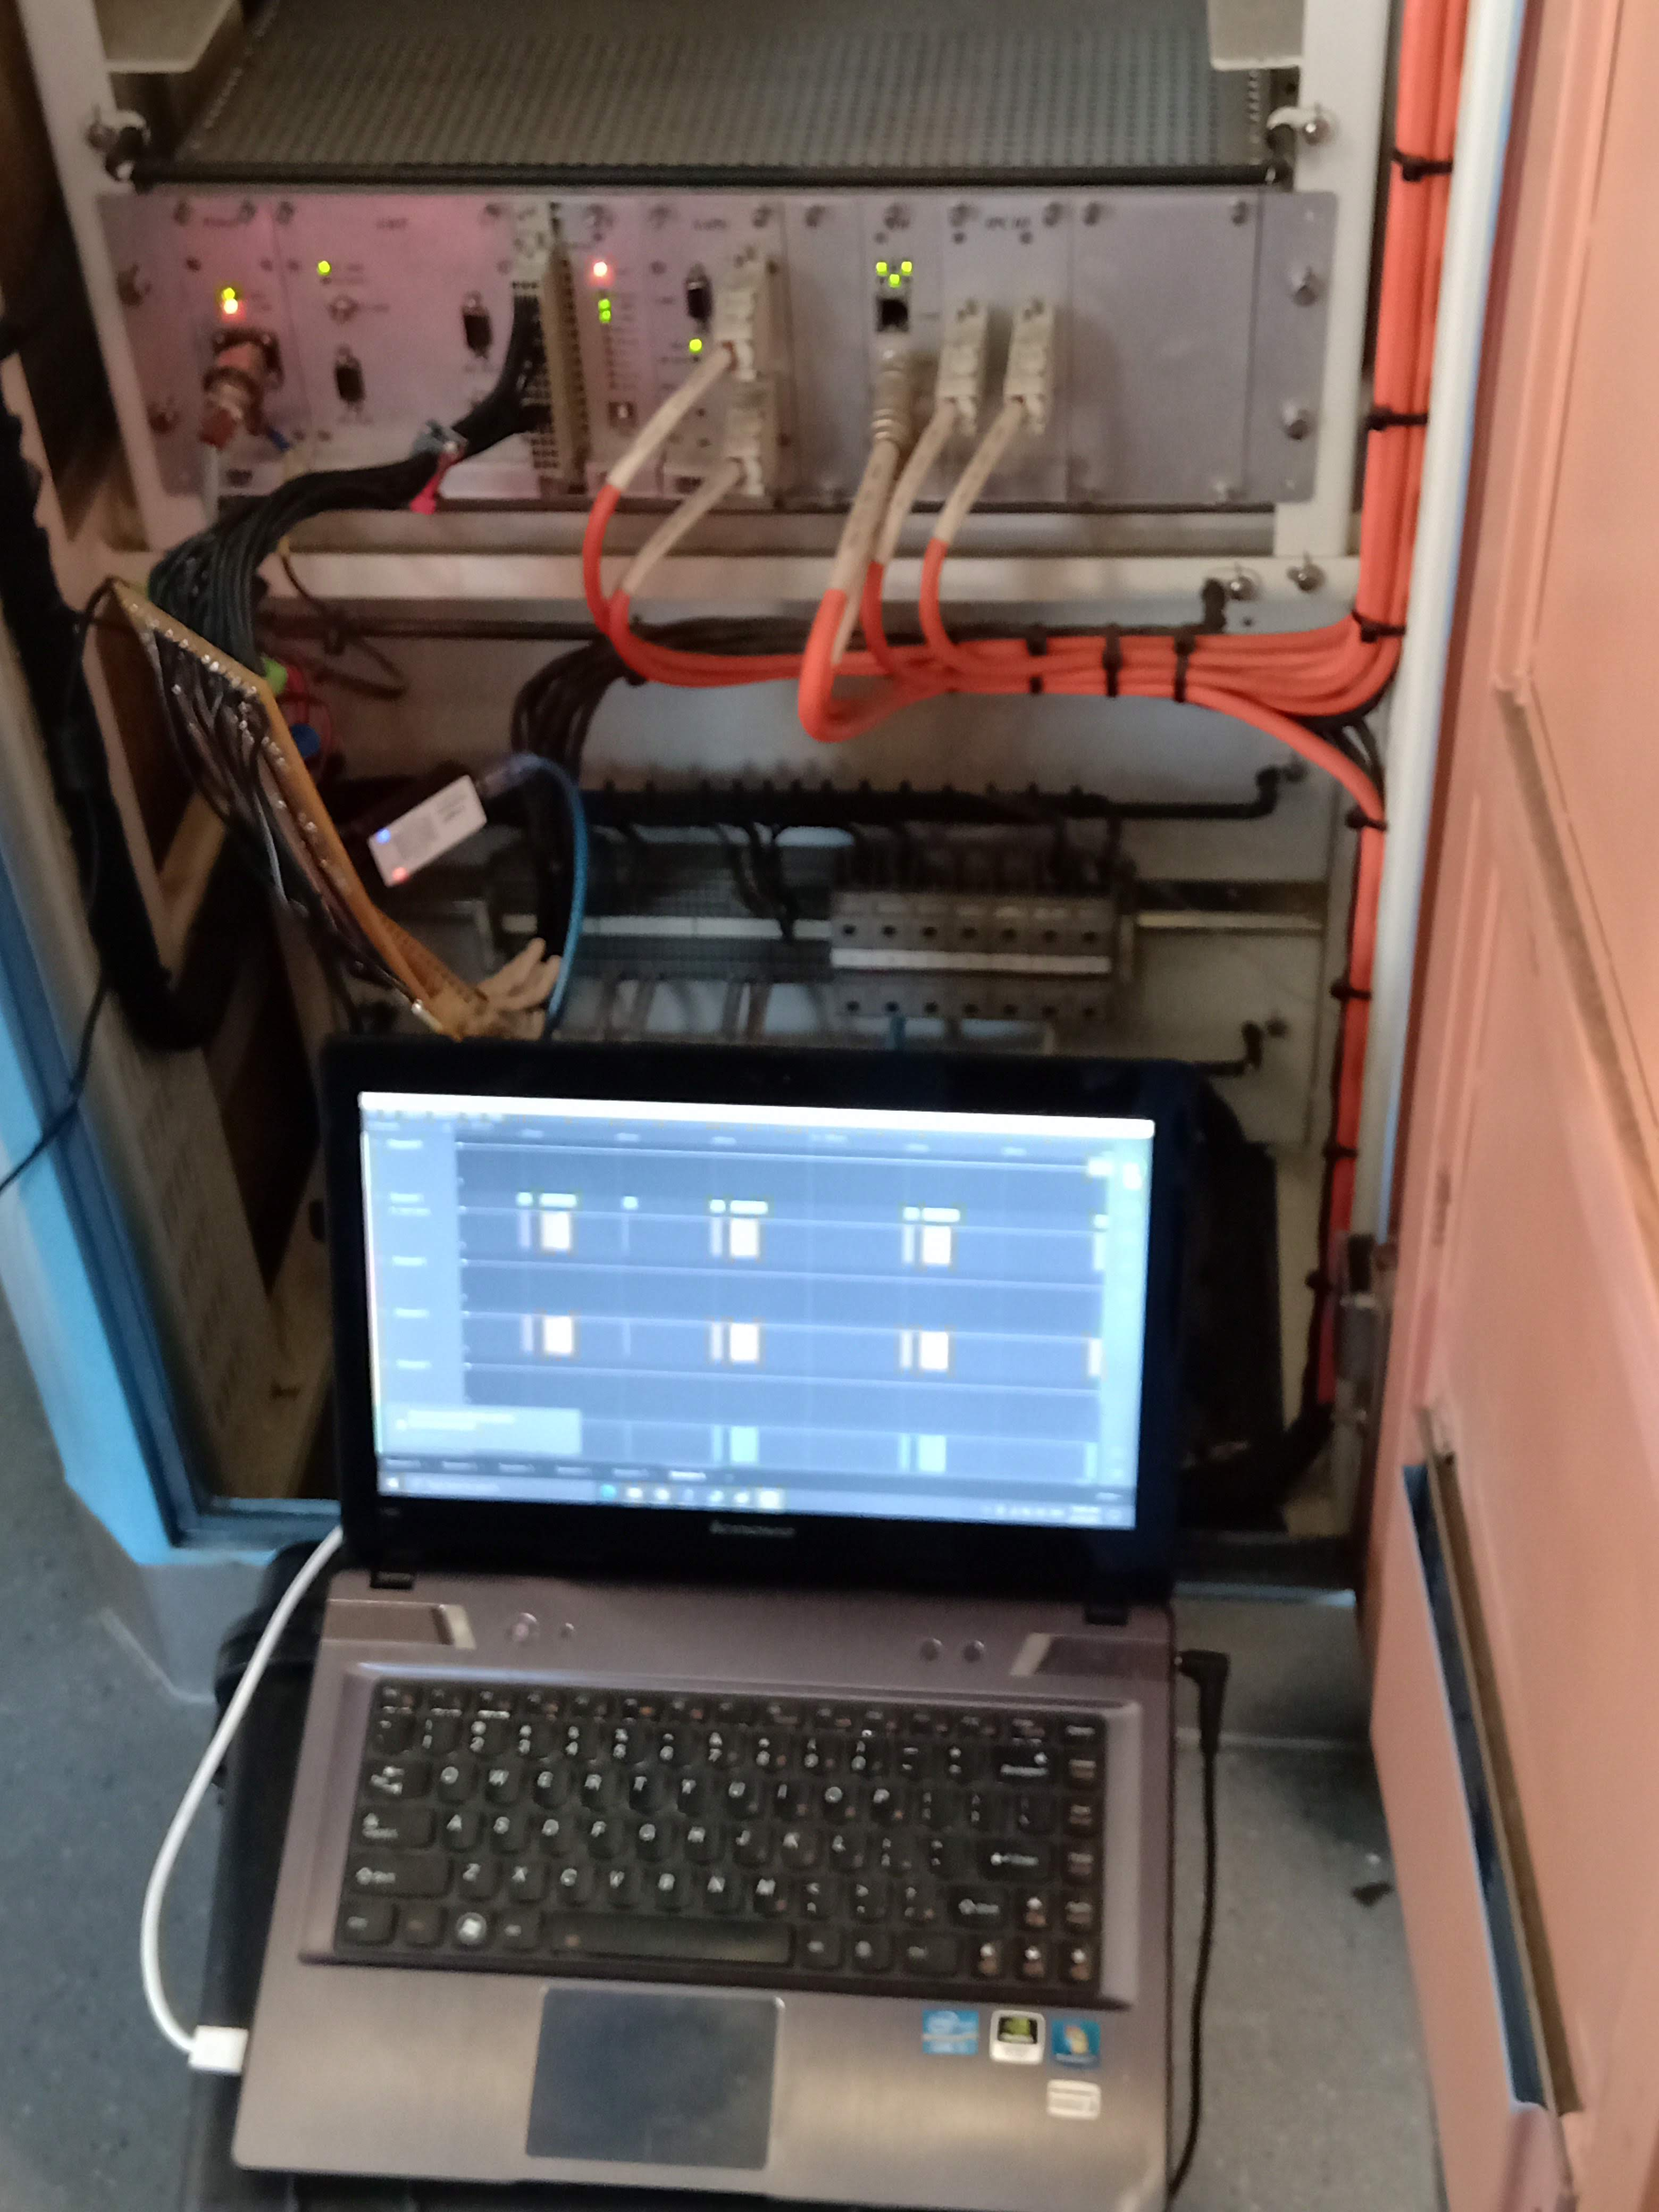
\includegraphics[width=1\textwidth]{./Pics/IMG_20210414_104653.jpg}
\caption{Fotografía del ensayo de análisis de protocolos de comunicación en una formación.}
\label{fig:sniffingPhoto}
\end{figure}

\section{Integración}

\end{document}


El sistema PIDS tiene la capacidad de presentar diversos mensajes de información al pasajero, como por ejemplo el nombre de la próxima estación, la temperatura actual, el tiempo estimado de arribo a destino, entre otros. Los mensajes se visualizan en carteles LED de 120 cm x 30 cm aproximadamente, usando matrices de punto LED de un solo color. La placa de control es compatible con manejadores de carteles LED comerciales, y también es compatible con la red eléctrica de 110 VDC del tren. El PIDS además cuenta con varios módulos adicionales, como son el sistema de sonido y el sistema de video entre otros. Cada módulo se compone de piezas de hardware específicas, distribuidas e interconectadas a lo largo del tren. En la figura \ref{fig:diagBloques} se presenta un diagrama de bloques del sistema PIDS. Se resalta en color los módulos de control incluidos en el alcance de este proyecto.

%\vspace{25px}

\begin{figure}[htpb]
\centering 
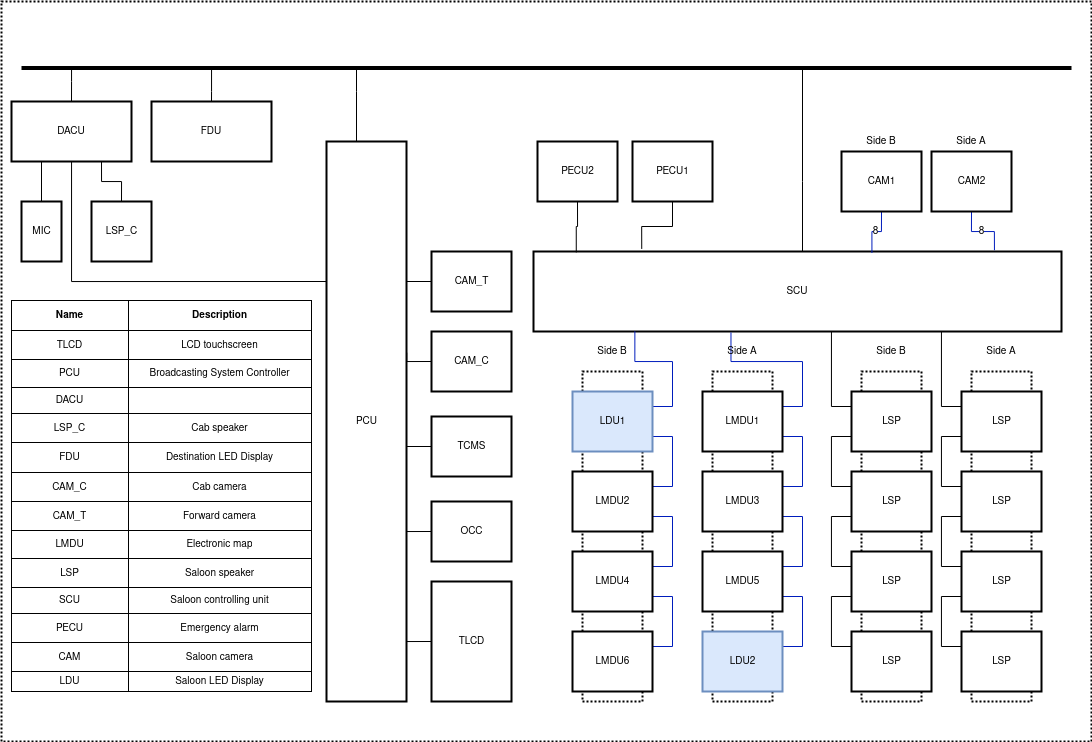
\includegraphics[width=.99\textwidth]{./Pics/RedPIDS.png}
\caption{}
\label{fig:diagBloques}
\end{figure}

\vspace{25px}

Este sistema también ofrece al personal técnico de SOFSE la capacidad de reemplazar placas existentes con alguna falla, configurar el nombre de distintos ramales usando el mismo hardware, y sirve de maqueta para capacitaciones.

Se propone en este trabajo diseñar y fabricar el controlador siguiendo las normas 50155 y 50126. La norma EN 50155 es la norma internacional que rige todos los equipos electrónicos de control, regulación, protección y suministro que se instalan en los vehículos ferroviarios. La norma EN 50126 define el ciclo de vida como: “estructura para la planificación, la gestión, el control y la supervisión de todos los aspectos de un sistema, incluido la fiabilidad, la disponibilidad, la mantenibilidad y la seguridad (RAMS), para entregar el producto adecuado al precio correcto dentro del plazo acordado.”


Este trabajo es continuación del trabajo final de la Carrera de Especialización en Sistemas Embebidos titulado Sistema de información visual para pasajeros, que se enmarca en un Proyecto de Desarrollo Estratégico (PDE), 'PDE\_15\_2020' de UBACyT titulado como “Sistema de monitoreo y gestión de la red TCN en formaciones ferroviarias”

\label{sec:backlog}

\subsection{UC-1} 
Como usuario quiero visualizar el nombre de la estación arribada.

\textbf{Descripción:} El sistema genera un mensaje que contiene información para el pasajero y se lo presenta en una marquesina LED.

\textbf{Disparadores:} El evento se inicia cuando el tren arriba a una 
estación.


